\documentclass[11pt, a4paper]{article}
\usepackage[T1]{fontenc}
\usepackage[utf8]{inputenc}
\usepackage[ngerman]{babel}
\usepackage[left=25mm, right=20mm, top=28mm, bottom=25mm,
            headheight=15pt, headsep=8mm, footskip=12mm]{geometry}
\usepackage{tgheros}
\renewcommand{\familydefault}{\sfdefault}
\usepackage[table]{xcolor}
\usepackage{titlesec}
\usepackage{enumitem}
\usepackage{fancyhdr}
\usepackage{tcolorbox}
\tcbuselibrary{skins}
\usepackage{graphicx}
\usepackage{booktabs}
\usepackage{tabularx}
\usepackage{array}
\usepackage[official]{eurosym}
\usepackage{siunitx}
\usepackage{parskip}
\usepackage{lastpage}
\usepackage{caption}
\usepackage[babel=true]{microtype}
\usepackage{hyperref}

% SI-Unit Setup & Euro-Deklaration
\sisetup{
  locale = DE,
  group-separator = {.},
  group-minimum-digits = 4,
  mode = text,
  range-phrase = --,
  range-units = single
}
\DeclareSIUnit{\EUR}{\text{\euro}}

% Corporate Design Colors Bündnis 90/Die Grünen
\definecolor{GruenPrimary}{HTML}{005425}   % Bündnisgrün / Tannengrün
\definecolor{GruenAccent}{HTML}{469A32}    % Maigrün
\definecolor{GruenLight}{HTML}{F0F6EF}     % Zarter grüner Hintergrund
\definecolor{GruenYellow}{HTML}{FFED00}    % Sonnenblumengelb
\definecolor{DarkText}{HTML}{1A1A1A}       % Dunkelgrau für Lesbarkeit
\definecolor{Grau}{HTML}{5E6A61}           % Nebentext, Beschriftungen
\definecolor{Linie}{HTML}{C8D5C7}          % Feine Trennlinien

\hypersetup{
    colorlinks=true,
    linkcolor=GruenPrimary,
    urlcolor=GruenPrimary,
    pdftitle={Haushaltsantrag 2027 - Bündnis 90/Die Grünen Plattling},
    pdfauthor={Martin Thoma - Stadtrat Plattling}
}

\urlstyle{same}

\DeclareCaptionFont{grau}{\color{Grau}}
\captionsetup{font={footnotesize,grau}, labelformat=empty,
              justification=raggedright, singlelinecheck=false, skip=4pt}

\linespread{1.05}
\arrayrulecolor{GruenPrimary}
\AtBeginDocument{\color{DarkText}}

% Kopf- und Fußzeile
\newcommand{\partei}{\textls[80]{BÜNDNIS 90/DIE GRÜNEN}}
\fancypagestyle{inhalt}{%
  \fancyhf{}
  \fancyhead[L]{\small\textcolor{GruenPrimary}{\bfseries\partei}\hspace{0.8em}\textcolor{Grau}{Stadtrat Plattling}}
  \fancyhead[R]{\small\textcolor{Grau}{Haushaltsantrag 2027}}
  \fancyfoot[L]{\footnotesize\textcolor{Grau}{Martin Thoma, Stadtrat}}
  \fancyfoot[R]{\footnotesize\textcolor{Grau}{Seite \thepage\ von \pageref*{LastPage}}}
  \renewcommand{\headrulewidth}{0.4pt}
  \renewcommand{\headrule}{\color{Linie}\hrule height \headrulewidth width \headwidth \vskip-\headrulewidth}
}
\fancypagestyle{titel}{%
  \fancyhf{}
  \fancyfoot[L]{\footnotesize\textcolor{Grau}{Martin Thoma, Stadtrat}}
  \fancyfoot[R]{\footnotesize\textcolor{Grau}{Seite \thepage\ von \pageref*{LastPage}}}
  \renewcommand{\headrulewidth}{0pt}
}
\pagestyle{inhalt}

% Überschriften: Nummer im grünen Quadrat
\titleformat{\section}[hang]
  {\normalfont\Large\bfseries\color{GruenPrimary}\raggedright}
  {\tikz[baseline=(n.base)]\node[fill=GruenPrimary, text=white, rounded corners=1.5pt,
     minimum width=1.6em, minimum height=1.6em, inner sep=0pt](n){\thesection};}
  {0.6em}{}
\titlespacing*{\section}{0pt}{0pt}{4mm}

% Kleine Versal-Beschriftung (Rubriken, Kennzahlen)
\newcommand{\rubrik}[1]{{\small\bfseries\color{GruenAccent}\textls[80]{\MakeUppercase{#1}}}}
\newcommand{\kennzahl}[1]{\leavevmode{\scriptsize\color{Grau}\textls[60]{\MakeUppercase{#1}}}}

% Maßnahme: Rubrik über der nummerierten Überschrift
\newcommand{\massnahme}[3]{%
  \rubrik{#1}\par\nobreak\vspace{1mm}%
  \section{#2}\label{#3}}

% Eckdaten-Leiste: Ansatz, Haushalt, Förderung
\newcommand{\eckdaten}[3]{%
  \begin{tcolorbox}[enhanced, colback=GruenLight, frame hidden, arc=1.5mm,
      left=5mm, right=5mm, top=2.5mm, bottom=2.5mm, before skip=0pt, after skip=5mm]
    \begin{tabularx}{\linewidth}{@{}p{0.22\linewidth} p{0.24\linewidth} >{\raggedright\arraybackslash}X@{}}
      \kennzahl{Ansatz 2027} & \kennzahl{Haushalt} & \kennzahl{Förderung / Finanzierung} \\[0.5mm]
      \leavevmode{\Large\bfseries\color{GruenPrimary}#1} & \bfseries #2 & \bfseries #3
    \end{tabularx}
  \end{tcolorbox}}

% Steckbrief: Beschriftung links, Text rechts
\newlist{steckbrief}{description}{1}
\setlist[steckbrief]{
  style=multiline,
  leftmargin=33mm,
  font=\small\bfseries\color{GruenPrimary},
  itemsep=3mm, parsep=1.5mm, topsep=0pt, partopsep=0pt
}

\setlist[itemize]{
  label=\textcolor{GruenAccent}{\raisebox{0.2ex}{\rule{0.42em}{0.42em}}},
  leftmargin=*, topsep=1mm, itemsep=1mm, parsep=0pt
}
\setlist[itemize,2]{label=\textcolor{GruenAccent}{\textendash}}
\setlist[enumerate]{
  label=\textcolor{GruenPrimary}{\bfseries\arabic*.},
  leftmargin=*, topsep=1mm, itemsep=1mm, parsep=0pt
}

\begin{document}

% ==============================================================================
% SEITE 1: ANSCHREIBEN & ÜBERSICHT
% ==============================================================================

\thispagestyle{titel}
\begin{tikzpicture}[remember picture, overlay]
  \fill[GruenPrimary] (current page.north west) rectangle ([yshift=-54mm]current page.north east);
  \fill[GruenYellow] ([yshift=-54mm]current page.north west) rectangle ([yshift=-55.5mm]current page.north east);
  \node[anchor=north west, inner sep=0pt, text width=165mm, align=left, text=white]
    at ([xshift=25mm, yshift=-14mm]current page.north west) {%
      {\small\bfseries\partei\hspace{0.8em}\textcolor{white!70!GruenPrimary}{\textls[80]{STADTRAT PLATTLING}}}\\[6mm]
      {\fontsize{34}{38}\selectfont\bfseries Haushaltsantrag\hspace{0.3em}2027}\\[3.5mm]
      {\large\color{white!85!GruenPrimary}Hitzeschutz \textperiodcentered{} Umweltbildung \textperiodcentered{} Erinnerungskultur \textperiodcentered{} Radverkehr}%
    };
\end{tikzpicture}

\vspace*{28mm}

{\small
\renewcommand{\arraystretch}{1.25}
\begin{tabularx}{\textwidth}{@{}>{\leavevmode\color{Grau}}p{12mm} X >{\leavevmode\color{Grau}}p{27mm} p{33mm}@{}}
An  & Erster Bürgermeister Hans Schmalhofer & Datum & \today \\
    & Stadtverwaltung Plattling & Abgabefrist & 1. Oktober 2026 \\
Von & Stadtrat Martin Thoma, Bündnis 90/Die Grünen & Verabschiedung & März 2027 \\
\end{tabularx}
}

\vspace{2mm}
{\color{Linie}\rule{\textwidth}{0.4pt}}

\textbf{Antrag zur Aufnahme von fünf Maßnahmen in den Haushaltsplan 2027}

Sehr geehrter Herr Bürgermeister Schmalhofer,\\
sehr geehrte Damen und Herren der Stadtverwaltung,

ich stelle hiermit folgenden Antrag zur Aufnahme in den Entwurf des
Haushaltsplans 2027:

\begin{tcolorbox}[enhanced, colback=GruenLight, frame hidden, sharp corners,
    borderline west={1mm}{0pt}{GruenPrimary},
    left=6mm, right=5mm, top=3.5mm, bottom=3.5mm, before skip=1mm, after skip=6mm]
\rubrik{Beschlussvorschlag}\par\smallskip
Der Stadtrat möge beschließen:
\begin{enumerate}
  \item Die nachfolgend aufgeführten Maßnahmen werden mit einem Gesamtvolumen von \qty{91500}{\EUR} in den Haushaltsentwurf für das Jahr 2027 aufgenommen und der fachlichen Prüfung durch die Verwaltung unterzogen.
  \item Die Verwaltung prüft vor der Mittelbewirtschaftung der investiven Positionen alle einschlägigen Förderzugänge – insbesondere \textit{KommKlimaFöR 2026}, die \textit{Bundesförderung für effiziente Gebäude (BEG)} und das \textit{Regionalbudget} – und reicht die Zuwendungsanträge fristgerecht vor Maßnahmebeginn ein.
\end{enumerate}
\end{tcolorbox}

\rubrik{Übersicht der beantragten Maßnahmen}

{\small
\renewcommand{\arraystretch}{1.2}
\begin{tabularx}{\textwidth}{@{}>{\bfseries\color{GruenPrimary}}l l l >{\raggedright\arraybackslash}X r r@{}}
\toprule
 & \textbf{Maßnahme} & \textbf{Haushalt}\textsuperscript{*} & \textbf{Förderung / Finanzierung} & \textbf{Ansatz 2027} & \textbf{S.} \\
\arrayrulecolor{Linie}\midrule
1 & Split-Klimageräte & Vermögenshaushalt & BEG EM, NKI-Kommunalrichtlinie & \qty{80000}{\EUR} & \pageref{m:klima} \\
2 & Nebelsprüh-System & Vermögenshaushalt & KommKlimaFöR 2026 (\SIrange{50}{90}{\percent}) & \qty{8000}{\EUR} & \pageref{m:nebel} \\
3 & Igel-Lehrpfad & Vermögenshaushalt & Naturschutzfonds, Regionalbudget & \qty{1000}{\EUR} & \pageref{m:igel} \\
4 & Stolpersteine & Verwaltungshaushalt & Patenschaften (Spenden) & \qty{1000}{\EUR} & \pageref{m:stolpersteine} \\
5 & Radwegweisung & Vermögenshaushalt & Eigenmittel & \qty{1500}{\EUR} & \pageref{m:radweg} \\
\arrayrulecolor{GruenPrimary}\midrule
 & \textbf{Gesamtvolumen} & & & \textbf{\qty{91500}{\EUR}} & \\
\bottomrule
\end{tabularx}

\smallskip
{\footnotesize\color{Grau}\textsuperscript{*}\,Die Zuordnung zu Verwaltungs- bzw. Vermögenshaushalt steht unter dem Vorbehalt der Prüfung durch die Kämmerei.}
}

\vfill

Mit freundlichen Grüßen

\vspace{8mm}

\textbf{Martin Thoma}\\
{\small\color{Grau}Stadtrat, Bündnis 90/Die Grünen Plattling}

\clearpage

% ==============================================================================
% SEITE 2: THEMA 1 - KLIMAGERÄTE
% ==============================================================================

\massnahme{Hitzeschutz}{Klimageräte in städtischen Gebäuden ersetzen und ergänzen}{m:klima}

\eckdaten{\qty{80000}{\EUR}}{Vermögenshaushalt}{BEG EM, NKI-Kommunalrichtlinie}

\begin{steckbrief}
  \item[Maßnahme] Reparatur bzw. Ersatz defekter Klimaanlagen in städtischen Gebäuden sowie Beschaffung und fachgerechte Installation von hocheffizienten Split-Klimageräten für besonders stark hitzebelastete Räume (insgesamt ca. 20 Räume). Reine Reparaturen werden als Unterhalt im Verwaltungshaushalt veranschlagt.
  \item[Priorisierung] \begin{enumerate}
      \item Reparatur bzw. Ersatz bestehender, defekter Anlagen.
      \item Räume für ehrenamtliche Einsatzkräfte, insbesondere die Aufenthalts- und Schulungsräume der Freiwilligen Feuerwehren Plattling, Pankofen und Pielweichs.
      \item Mittelschule (Preysingstraße) – mit Fokus auf Dachgeschosse und nach Süden/Westen ausgerichtete Klassenzimmer.
    \end{enumerate}
  \item[Sperrvermerk] Qualifizierter Sperrvermerk: Die Freigabe der Haushaltsmittel erfolgt nach Vorlage und Genehmigung des Raum- und Umsetzungskonzepts im Haupt- und Finanzausschuss bzw. Bauausschuss.
  \item[Förderung] \begin{itemize}
      \item \textit{BAFA / KfW Bundesförderung für effiziente Gebäude (BEG EM):} Förderung von energieeffizienter Anlagentechnik bei Nutzung von Split-Geräten mit Wärmepumpenfunktion und natürlichen Kältemitteln (z.\,B. R290/Propan).
      \item \textit{Kommunalrichtlinie (NKI):} Unterstützung bei investiven Maßnahmen zum sommerlichen Wärmeschutz an Schulen.
    \end{itemize}
  \item[Arbeitsauftrag] Bestandsaufnahme der defekten Anlagen im städtischen Gebäudebestand; Ermittlung des Bedarfs in den Feuerwehrhäusern in Abstimmung mit den Kommandanten sowie in der Mittelschule mit der Schulleitung; Prüfung, ob weitere städtische Räume regelmäßig von ehrenamtlichen Organisationen genutzt werden; Klärung der baulichen Voraussetzungen und Förderantragsfristen.
  \item[Begründung] Defekte Anlagen fallen gerade an Hitzetagen aus, ihre Instandsetzung sichert den Wert bereits getätigter Investitionen. Die ehrenamtlichen Einsatzkräfte der Feuerwehren leisten ihren Dienst in der Freizeit, oft direkt nach Einsätzen in schwerer Schutzkleidung. Erträgliche Aufenthalts- und Schulungsräume sind ein Zeichen der Wertschätzung und stärken das Ehrenamt. Extreme Hitzeperioden beeinträchtigen zudem die Konzentrations-, Lern- und Leistungsfähigkeit von Schülerinnen, Schülern und Lehrkräften messbar. Durch moderne Wärmepumpentechnik können die Anlagen in den Übergangsmonaten hocheffizient zum Heizen genutzt werden.
\end{steckbrief}

\clearpage

% ==============================================================================
% SEITE 3: THEMA 2 - NEBELSPRÜH-SYSTEM
% ==============================================================================

\massnahme{Hitzeschutz}{Mobil-flexibles Nebelsprüh-System zur Hitzeminderung}{m:nebel}

\eckdaten{\qty{8000}{\EUR}}{Vermögenshaushalt}{KommKlimaFöR 2026 (\SIrange{50}{90}{\percent})}

\begin{steckbrief}
  \item[Maßnahme] Beschaffung eines mobil-flexiblen Nebelsprüh-Systems zur Verdunstungskühlung im öffentlichen Raum (technische Orientierung an Systemen wie \textit{Water Oasis} in Fürth). Das System benötigt keinen Stromanschluss.
  \item[Standorte] \begin{itemize}
      \item \textit{Hauptstandort:} Spielplatz Preysingstraße / Sterngasse (dicht bebauter Bereich).
      \item \textit{Mobile Nutzung:} temporäre Umsetzung zu innerstädtischen Veranstaltungen (z.\,B. Volksfestplatz, Nibelungenfest).
    \end{itemize}
  \item[Kosten] ca. \qty{5000}{\EUR} Anschaffung, ca. \qty{3000}{\EUR} Installation, Montage und Wasseranschluss.
  \item[Förderung] \textit{KommKlimaFöR 2026 (Freistaat Bayern):} Explizite Förderung von investiven Klimaanpassungsmaßnahmen wie „klimafreundlichen Wasseranlagen zur Kühlung der Umgebung“ auf öffentlichen Plätzen und Spielplätzen. Reguläre Förderquote bis zu \SI{50}{\percent} (bei Bedarf bis zu \SI{90}{\percent}).
  \item[Arbeitsauftrag] Technische Prüfung des örtlichen Wasseranschlusses am Spielplatz sowie Einreichung des Förderantrags über die Fördermanagementplattform Bayern (FMP) vor Auftragsvergabe.
  \item[Begründung] Feine Hochdruck-Verdunstungskühlung senkt die gefühlte Umgebungstemperatur an Hitzetagen spürbar ab, ohne Nässe zu erzeugen, und benötigt dabei nur minimale Wassermengen. Die Anlage schützt im Bereich des Spielplatzes täglich zahlreiche Kinder und Eltern vor akuter Hitzebelastung.
\end{steckbrief}

\clearpage

% ==============================================================================
% SEITE 4: THEMA 3 - IGEL-LEHRPFAD
% ==============================================================================

\massnahme{Umweltbildung}{Errichtung eines Igel-Lehrpfades am Mühlbach}{m:igel}

\eckdaten{\qty{1000}{\EUR}}{Vermögenshaushalt}{Naturschutzfonds, Regionalbudget}

\begin{steckbrief}
  \item[Maßnahme] Beschaffung des praxiserprobten, kindgerechten Lehrtafel-Sets des Vereins \textit{Pro Igel e.V.} und dauerhafte Aufstellung am Mühlbach.
  \item[Standort] Mühlbach-Promenade, nach Möglichkeit im Bereich der neuen Kindertagesstätte an der Steinfeldstraße (Pielweichs), die ebenfalls am Mühlbach liegt. So kann der Kindergarten den Lehrpfad im Alltag mitnutzen.
  \item[Kosten] \qty{1000}{\EUR} Sachkosten für Beschilderung und Infotafeln; Fundamente, Pfosten und Montage übernimmt der städtische Bauhof in Eigenleistung.
  \item[Förderung] \begin{itemize}
      \item \textit{Bayerischer Naturschutzfonds / Umweltstiftungen:} Förderung lokaler Projekte zur Natur- und Artenschutzbildung im Siedlungsraum.
      \item \textit{ILE-Regionalbudget / Kleinprojekte:} Bis zu \SI{80}{\percent} Fördersatz für gemeinwohlorientierte Kleinmaßnahmen im ländlichen Raum.
    \end{itemize}
  \item[Arbeitsauftrag] Einplanung der benötigten Bauhof-Kapazitäten für Fundamente, Pfosten und Montagearbeiten sowie Festlegung des Standorts in Abstimmung mit der Planung der Kindertagesstätte und der genauen Tafelstandorte.
  \item[Begründung] Der Igel steht als Leitart für einen artenreichen Garten- und Siedlungsraum, gerät jedoch zunehmend unter Druck. Ein Igel-Lehrpfad schafft mit minimalem finanziellem Aufwand ein dauerhaftes, interaktives Umweltbildungsangebot für Spaziergänger, Familien, Kindergärten und Schulklassen entlang einer der meistfrequentierten Naherholungsachsen Plattlings.
\end{steckbrief}

\clearpage

% ==============================================================================
% SEITE 5: THEMA 4 - STOLPERSTEINE
% ==============================================================================

\massnahme{Erinnerungskultur}{Stolpersteine für Plattlinger Opfer des Nationalsozialismus}{m:stolpersteine}

\eckdaten{\qty{1000}{\EUR}}{Verwaltungshaushalt}{Patenschaften (Spenden)}

\begin{steckbrief}
  \item[Maßnahme] \begin{enumerate}
      \item Grundsatzbeschluss des Stadtrats, der die Verlegung von Stolpersteinen im öffentlichen Straßenraum genehmigt. Die Steine gehen nach der Verlegung in das Eigentum der Stadt über.
      \item Feststellung der betroffenen Personen und Familien sowie ihrer letzten frei gewählten Wohnadressen durch Ehrenamtliche und Schulen, unterstützt durch das Stadtarchiv; Kontaktaufnahme mit den Nachfahren. Erste Hinweise gibt es zu den Familien Schilling, Behr und Kohn, voraussichtlich in der Luitpoldstraße und der Reiterstraße (siehe folgende Seite).
      \item Herstellung und Verlegung der Steine im Rahmen einer öffentlichen Gedenkveranstaltung, z.\,B. über das Projekt „Stolpersteine“ von Gunter Demnig (\url{https://www.stolpersteine.eu}).
    \end{enumerate}
  \item[Kosten] ca. \qty{1000}{\EUR} für Herstellung und Verlegung der Steine (nach ersten Hinweisen etwa acht). Richtwert: \qty{120}{\EUR} je Stein einschließlich Verlegung beim Projekt von Gunter Demnig. Die Recherche übernehmen Ehrenamtliche; die Verlegestellen bereitet der Bauhof in Eigenleistung vor.
  \item[Refinanzierung] Patenschaften von Bürgerinnen und Bürgern, Vereinen, Firmen und Schulen gegen Zuwendungsbestätigung. Die Stadt finanziert die Steine vor, damit die Verlegung nicht vom Spendeneingang abhängt.
  \item[Begründung] Stolpersteine erinnern an Menschen, die in der Zeit des Nationalsozialismus verfolgt, vertrieben oder ermordet wurden – vor dem Haus, in dem sie zuletzt frei gelebt haben, mitten im Alltag. Sie geben den Opfern ihre Namen zurück und machen sichtbar, dass Ausgrenzung und Verfolgung nicht anonym und nicht irgendwo anders geschahen, sondern in der eigenen Nachbarschaft. Da es kaum noch Zeitzeuginnen und Zeitzeugen gibt, gewinnen solche Orte an Bedeutung: Sie halten wach, wohin Hass und Ausgrenzung führen können, und stärken das Bewusstsein für Demokratie und Menschenwürde. Die Recherche zu den Biografien bietet Schülerinnen und Schülern zudem die Möglichkeit, sich selbst mit der Geschichte ihrer Stadt auseinanderzusetzen.
\end{steckbrief}

\clearpage

\rubrik{Stolpersteine: Erste Hinweise}\footnote{Quellen: M.~Westerholz, \emph{Plattling und das missglückte KZ-Gedenken}, haGalil, 21.\,01.\,2025; Liste der Stolpersteine in Regensburg (Wikipedia). Die Angaben sind im Zuge der Recherche zu prüfen.}

Veröffentlichte Quellen nennen bisher die folgenden Personen. Welche Personen und Familien berücksichtigt werden, klärt die Recherche; je Person wird ein Stein verlegt.

{\small
\renewcommand{\arraystretch}{1.35}
\begin{tabularx}{\textwidth}{@{}l c >{\raggedright\arraybackslash}X@{}}
\toprule
\textbf{Name} & \textbf{Jahrgang} & \textbf{Schicksal} \\
\arrayrulecolor{Linie}\midrule
Moritz Schilling & 1859 & starb vermutlich in einem Versteck in Plattling \\
\midrule
Max Behr & 1889 & 1937 Flucht nach New York \\
Julie Behr, geb.\ Schilling & 1894 & 1937 Flucht nach New York \\
Heinz Behr & 1921 & 1937 Flucht nach New York \\
Gerda Behr & 1924 & 1937 Flucht nach New York \\
Helmut Behr & 1934 & 1937 Flucht nach New York \\
\midrule
Oskar Kohn & 1877 & 1936 Umzug nach Regensburg, 1942 nach Piaski deportiert und ermordet \\
Eugenie Kohn, geb.\ Steinreich & 1882 & 1936 Umzug nach Regensburg, 1942 nach Piaski deportiert und ermordet \\
\arrayrulecolor{GruenPrimary}\bottomrule
\end{tabularx}
}

Für das Ehepaar Kohn liegen seit 2010 Stolpersteine in Regensburg (Ludwigstraße~5). Ob zusätzlich am früheren Plattlinger Wohnort Steine verlegt werden, ist im Zuge der Recherche zu klären. Die Verlegeorte (voraussichtlich Luitpoldstraße und Reiterstraße) werden im Zuge der Recherche festgelegt.

\vspace{4mm}
\begin{minipage}[b]{0.42\textwidth}
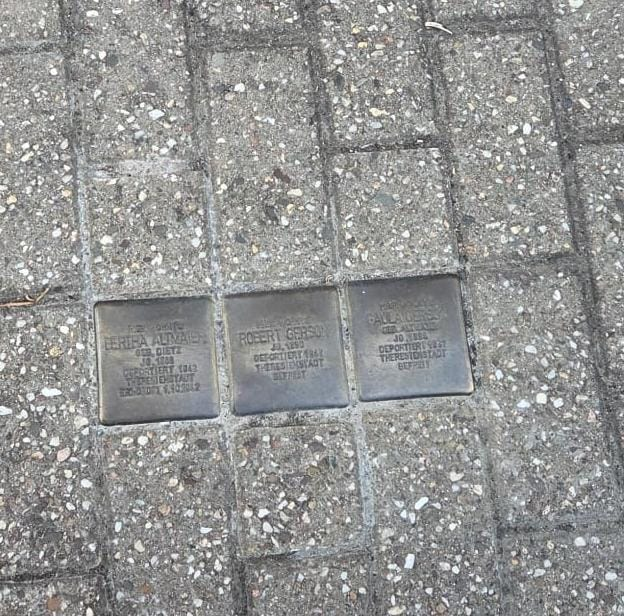
\includegraphics[width=\linewidth]{stolpersteine-Frankfurt.jpg}
\end{minipage}\hspace{5mm}%
\begin{minipage}[b]{0.40\textwidth}
\captionof{figure}{Beispiel: Stolpersteine in Frankfurt am Main. Jeder Stein ist \qtyproduct{10 x 10}{cm} groß und trägt eine Messingplatte mit Namen, Jahrgang und Schicksal.}
\end{minipage}

\clearpage

% ==============================================================================
% SEITE 6: THEMA 5 - RADWEGWEISUNG
% ==============================================================================

\massnahme{Radverkehr}{Radwegweisung zwischen Plattling und Deggendorf verbessern}{m:radweg}

\eckdaten{\qty{1500}{\EUR}}{Vermögenshaushalt}{Eigenmittel}

\begin{steckbrief}
  \item[Maßnahme] Pfeilwegweiser mit Zielangabe (und Entfernung) an vier Knotenpunkten der Radverbindung Plattling–Pankofen–Mainkofen–Deggendorf. Die Gestaltung richtet sich nach dem Radverkehrsnetz des Landkreises Deggendorf.
  \item[Standorte] \begin{enumerate}
      \item \textit{Pankofen Mühle, bei Weiß Holzbau / Lidl:} Hier teilt sich der Radweg: geradeaus über Schiltorn, links über Mainkofen. Der bestehende Wegweiser zeigt nur geradeaus und nennt kein Ziel (siehe Foto). Ein Wegweiser „Deggendorf“ soll auf die Route über Mainkofen hinweisen, die insbesondere abends die bessere Wahl ist.
      \item \textit{Gabelung Pankofen Hauptstraße / Pankofen Dorfstraße:} ein Wegweiser.
      \item \textit{Bahnhof Pankofen:} je ein Wegweiser in beide Fahrtrichtungen (Deggendorf bzw.\ Plattling).
      \item \textit{Radweg Richtung Mainkofen, Abzweigung zur St~2124:} ein Wegweiser.
    \end{enumerate}
\end{steckbrief}

\vspace{3mm}
\begin{minipage}[t]{0.53\textwidth}
\vspace{0pt}
\rubrik{Kostenschätzung}\par\vspace{1mm}

{\footnotesize
\renewcommand{\arraystretch}{1.3}
\begin{tabularx}{\linewidth}{@{}>{\raggedright\arraybackslash}X r@{}}
\toprule
\textbf{Position} & \textbf{Kosten} \\
\arrayrulecolor{Linie}\midrule
5 Pfeilwegweiser (Alu, reflektierend, Ziel/km, inkl.\ Schellen), je ca.\ \qty{200}{\EUR} & \qty{1000}{\EUR} \\
1 neuer Rohrpfosten inkl.\ Bodenhülse (alle übrigen Standorte: vorhandene Pfosten) & \qty{150}{\EUR} \\
Kleinmaterial, Zwischenwegweiser, Reserve & \qty{350}{\EUR} \\
Montage (Bauhof, ca.\ ½ Arbeitstag) & Eigenleistung \\
\arrayrulecolor{GruenPrimary}\midrule
\textbf{Summe} & \textbf{\qty{1500}{\EUR}} \\
\bottomrule
\end{tabularx}
}
\end{minipage}\hfill
\begin{minipage}[t]{0.43\textwidth}
\vspace{0pt}
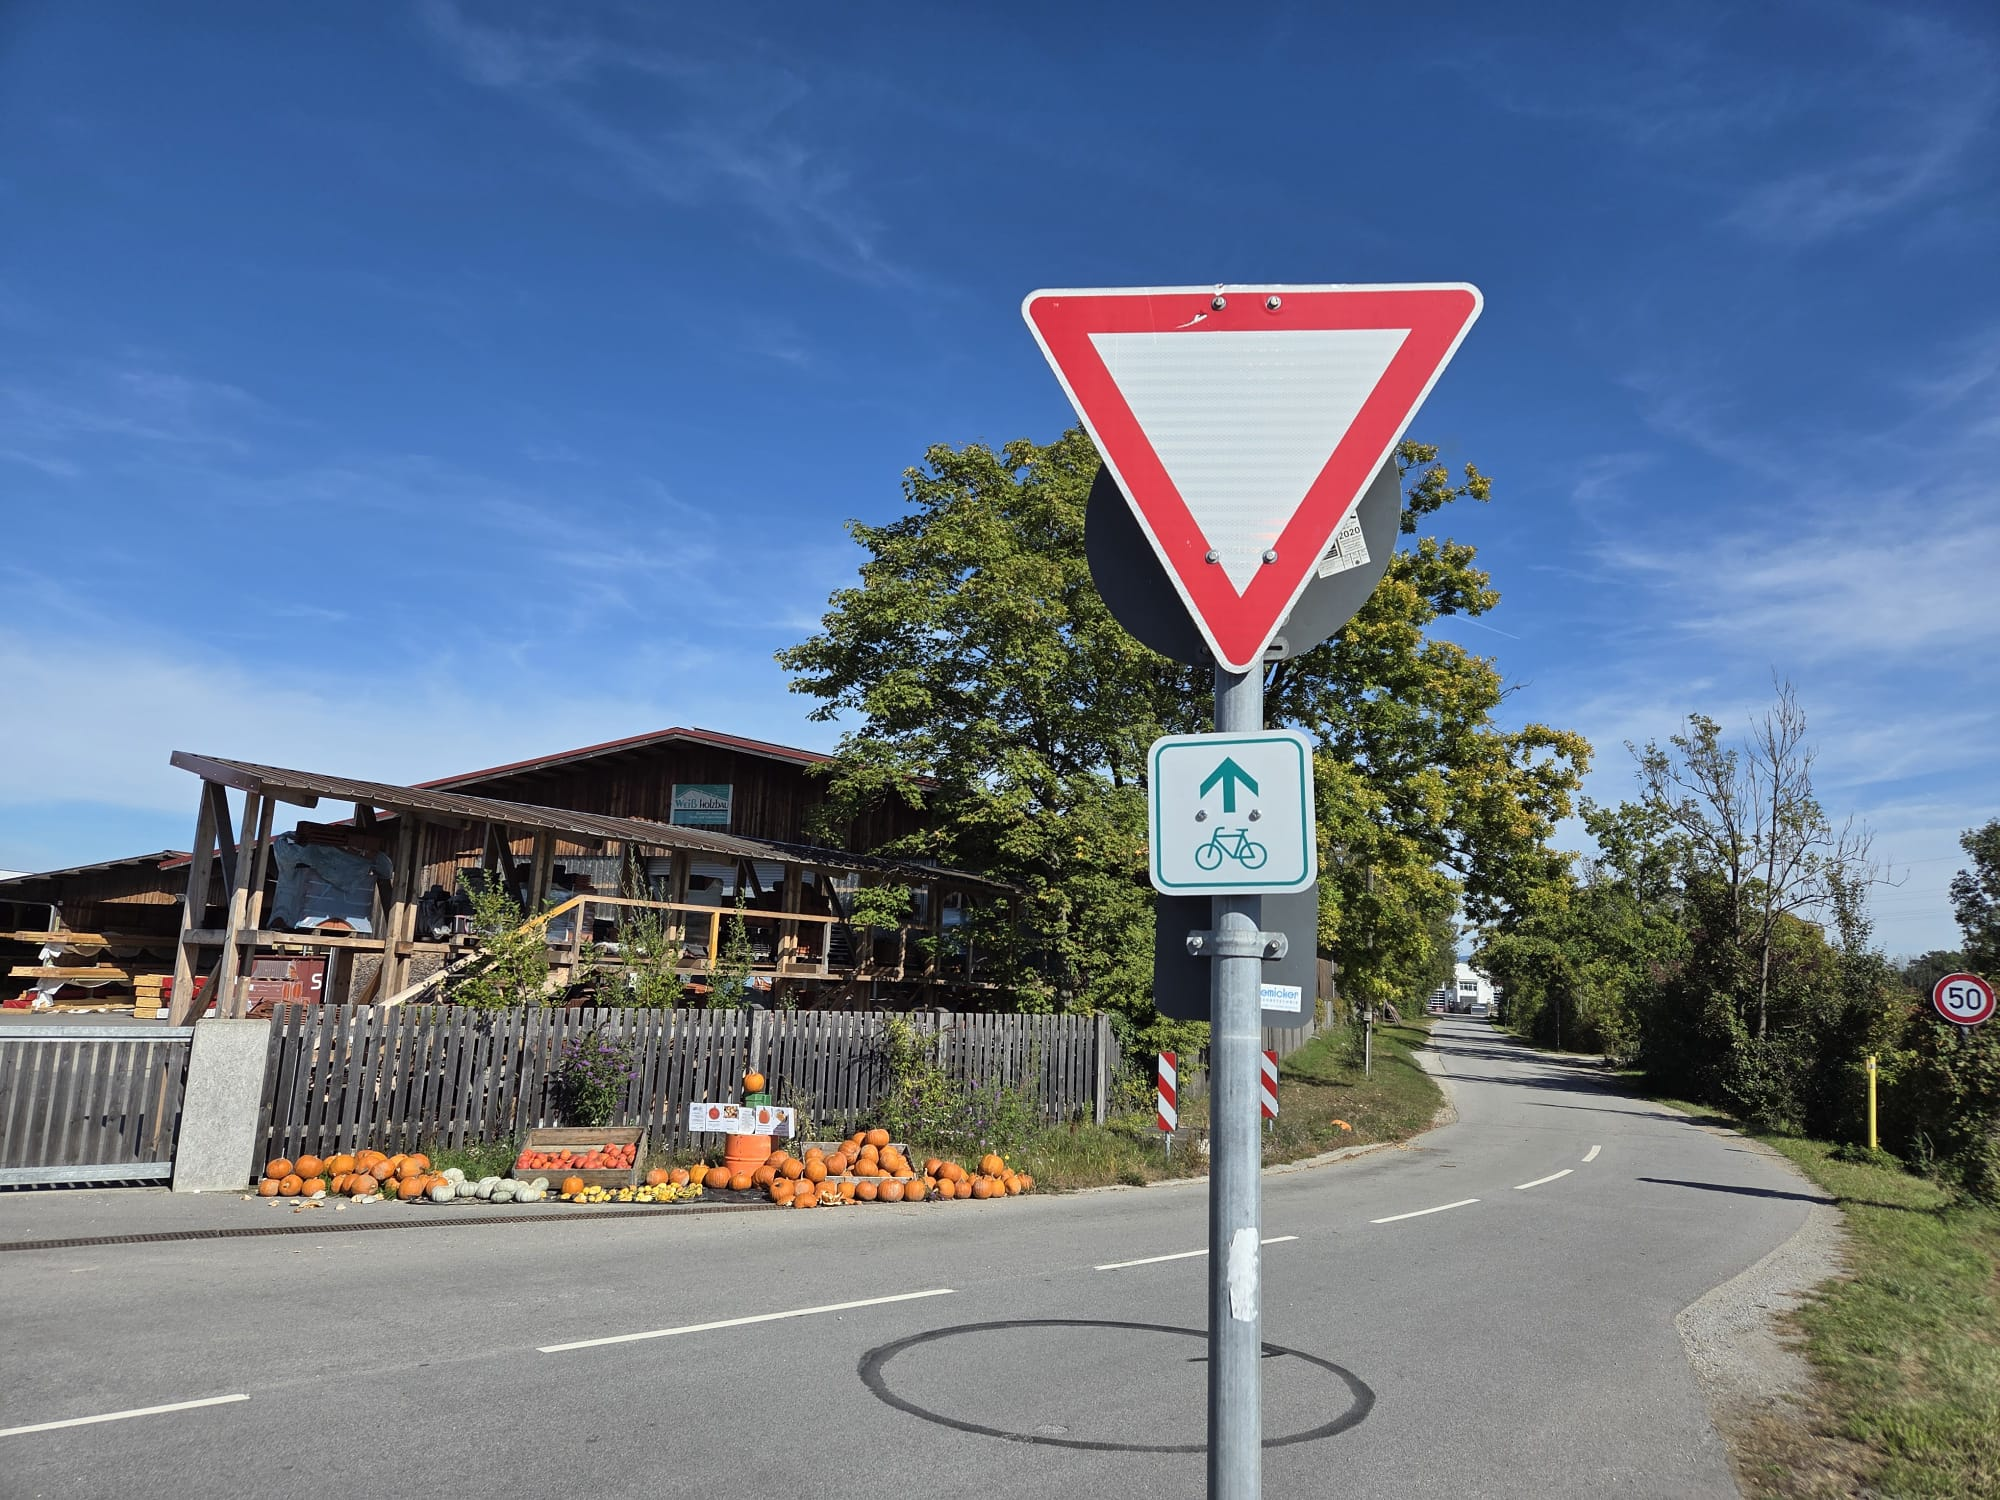
\includegraphics[width=\linewidth]{Fahrradschild-mit-name-bei-Lidl.jpeg}
\captionof{figure}{Wegweiser bei Weiß Holzbau / Lidl: Pfeil geradeaus (über Schiltorn) ohne Ziel; die Route über Mainkofen zweigt links ab.}
\end{minipage}

\vspace{3mm}
\begin{steckbrief}
  \item[Arbeitsauftrag] Festlegung der genauen Standorte und Zielangaben in Abstimmung mit dem Landkreis Deggendorf (einheitliches Radverkehrsnetz) sowie für den Standort an der St~2124 mit dem Staatlichen Bauamt. Bis auf einen Standort werden vorhandene Pfosten mitgenutzt.
  \item[Begründung] Die Strecke über Pankofen ist eine wichtige Alltagsverbindung zwischen Plattling, dem Bahnhof Pankofen, dem Bezirksklinikum Mainkofen und Deggendorf. An mehreren Abzweigungen fehlt eine Zielangabe, sodass Radfahrende leicht falsch abbiegen und Umwege fahren. Wenige Schilder machen die Verbindung für Radfahrende deutlich einfacher nutzbar.
\end{steckbrief}

\end{document}
